%----------------------------------------------------------------------------
\chapter{\AudioBasics}
%----------------------------------------------------------------------------

\begin{comment} 
Annak érdekében, hogy a későbbi fejezetekben a hangtechnikai rendszerek működését és tervezését megérthessük,
először szükséges a hangtechnikai alapok ismerete. Ez a fejezet a későbbi fejezetekben használt alapfogalmakat definiálja röviden és tömören.

%----------------------------------------------------------------------------
\section{Mikrofon típusok}
%----------------------------------------------------------------------------

A mikrofon egy eszköz, amely az akusztikus energia hangterét elektromos energiává alakítja át.
Az eszköz érzékelheti a hangnyomást vagy a hangnyomás gradienst, amely arányos a hangsebességgel (mindkettő kombinációja a hangintenzitásnak).
Négy különböző átalakítótípus létezik, amelyeket reciprok transzducerekként használhatunk mikrofonokhoz:

% ----------------------------------------------------------------------------
\begin{itemize}
    \item Kapacitív transzducer
    \item Piezoelektromos transzducer
    \item Dinamikus transzducer
    \item Mágneses transzducer
\end{itemize}
% ----------------------------------------------------------------------------

Az említett összes transzducer lehetővé teszi a mechanikai rezgések elektromos rezgésekké történő átalakítását,
miközben különböző elveket követnek. Az első kettő esetében az elektromos mező változása
van használatban, míg az utolsó kettő esetében egy vezetőben keletkező áram indukciója a mágneses térben történő vezetékmozgás révén,
vagy a mágneses fluxus változása egy tekercsen. 
Elsősorban a négy említett transzducer közül kettőt a kapacitív és a dinamikus transzducert
használjuk gyakorlati jelentőséggel a rendezvénytechnikában.

% ----------------------------------------------------------------------------
\subsection{Dinamikus mikrofon}
% ----------------------------------------------------------------------------

A dinamikus mikrofonok a legelterjedtebb mikrofonok a hangtechnikában.
A hangnyomás mechanikai rezgéseit alakítják elektromos jelekké, elve, hogy egy membrán mely egy tekercsre van rögzítve, és ez mágneses mezőben mozog.
A membrán rezgése a tekercsben elektromos feszültséget indukál, amely a hangjelet reprezentálja.
Nagyon strapabíróak és megbízhatóak, széles körben használják őket élő hangosításban és stúdiótechnikában.
Hátránya a kisebb frekvenciaátvitel és a nagyobb torzítás.
Az egyik legismertebb dinamikus mikrofon a Shure SM57, amely egy nagyon népszerű mikrofon a hangtechnikában, és sokféle alkalmazásban használják.

% ----------------------------------------------------------------------------
\begin{figure}[H]
    \centering
    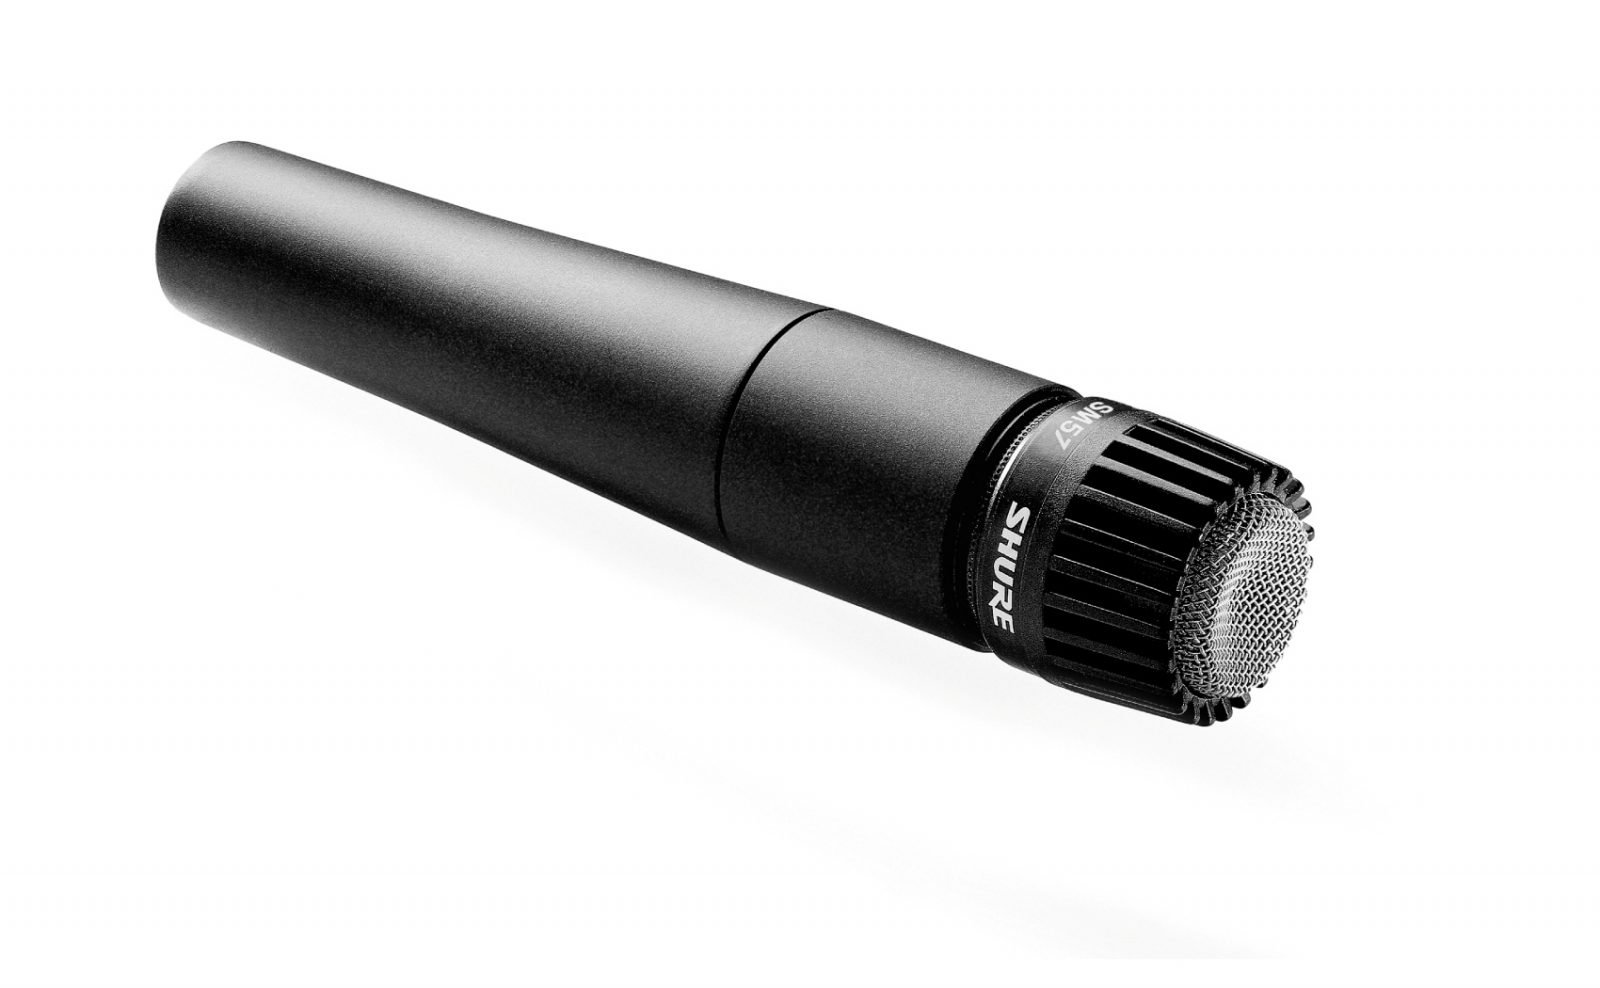
\includegraphics[width=0.3\textwidth]{figures/shure-sm57.jpg}
    \caption{Shure SM57 dinamikus mikrofon}
    \label{fig:shure_sm57}
\end{figure}
% ----------------------------------------------------------------------------

 
% ----------------------------------------------------------------------------
\subsection{Kondenzátor mikrofon}
% ----------------------------------------------------------------------------

A kondenzátor mikrofonok a nagyobb frekvenciaátvitellel rendelkező mikrofonok, és a nagyobb dinamikatartományt is képesek lefedni.
A hangnyomás a membrán rezgéseit egy kondenzátorban változó kapacitásként alakítja át, amelynek egyik eleme a membrán, a másik pedig egy fix elektromosan töltött lemez.
A membrán rezgései a kapacitás változását okozzák, amely a hangjelet reprezentálja.
A kondenzátor mikrofonok nagyon érzékenyek, és nagyon jó hangminőséget biztosítanak.
Azonban a kondenzátor mikrofonoknak van néhány hátránya is, például az áramellátás szükségessége, a magasabb ár és a nagyobb méretek.
Egy példa a kondenzátor mikrofonra a Shure SM137 kondenzátor mikrofon, amely egy elterjed mikrofon a hangtechnikában.

% ----------------------------------------------------------------------------
\begin{figure}[H]
    \centering
    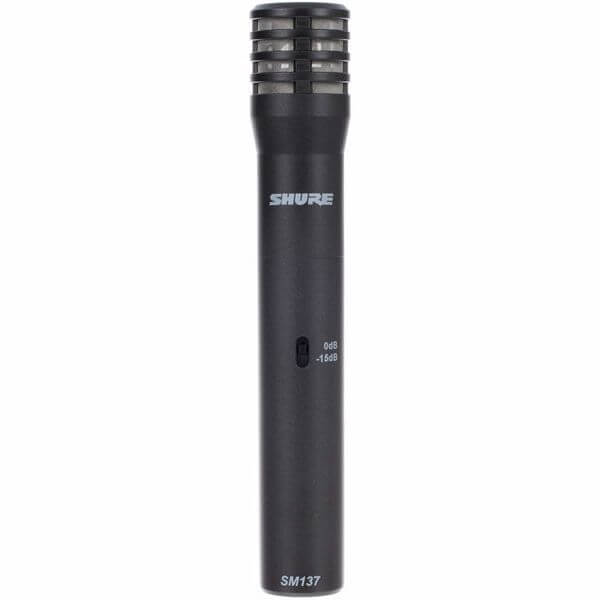
\includegraphics[width=0.3\textwidth]{figures/shure-sm137.jpg}
    \caption{Shure SM137 kondenzátor mikrofon}
    \label{fig:shure_sm137}
\end{figure}
% ----------------------------------------------------------------------------
\end{comment}

% ⛔📝 TODO: Merge text formatting and content integration check

%----------------------------------------------------------------------------
\section{Az analóg kezdetek} % Kezdeti analóg rendszerek, skálázhatósági hátrányok, analog rendszerek korlátai, működési alapelvek, technológiai háttér  
%----------------------------------------------------------------------------
Az analóg hangrendszerek története az audio technológia hajnalára nyúlik vissza. 
Az ilyen rendszerek alapját az elektromos analóg jelek képezik, amelyek az akusztikus hangot elektromos árammá alakítják,
a hangjelet közvetlenül, torzítás nélkül próbálják átadni az erősítőnek majd ezáltal hangszóróknak.
Az analóg rendszerek egyik legfontosabb alapelve az elektromos jelek folyamatos feldolgozása. 
A hangot analóg módon rögzítik, és az áramkörök szigorú tervezése biztosítja, hogy az eredeti akusztikus jel minél pontosabban tükröződjön az outputban.
A legnagyobb hátrány az analóg rendszerek skálázhatóságában rejlik. 
Ahogy a rendszer bonyolultsága nőtt, úgy a karbantartás és az állandó finomhangolás is egyre több problémát okozott. 
Az analóg technológiáknál a jel erősítése és kezelése gyakran jelentős torzulásokat és zajokat okozott, amelyeket nehéz volt kezelni.
A kábelezést tekintve sem volt egy leányálom az analóg rendszerek használata, mivel a nagyobb távolságokon a jel torzulása és a zajok könnyen bekerülhettek a rendszerbe.
Egy sokcsatornás produkciónál szép spagettiláncokat is eredményezett, még a legtapasztaltabb hangmérnökök számára is kihívást jelentett. 
Továbbá, a rendszer hibái nem mindig voltak könnyen diagnosztizálhatók, ami a szervizelési időket jelentősen megnövelte.
A hangrendszerek technológiai hátterét tekintve, az analóg rendszerekben a transzformátorok, kondenzátorok és ellenállások kulcsszerepet játszottak. 
Ezek az alkatrészek feleltek a jel szűréséért, erősítéséért és átalakításáért. 
Azonban ezek az elemek gyakran voltak érzékenyek a környezeti hatásokra, mint például a hőmérséklet-ingadozások és a páratartalom, 
amelyek további kihívások elé állították a hangmérnököket.
%----------------------------------------------------------------------------
\section{Digitális térhódítás} % Miért digitális irányba fejlesztünk és halad az ipar? Miért jobb mint az analog? 
%----------------------------------------------------------------------------
A digitális technológia térhódítása a professzionális audio rendszerekben jelentős paradigmaváltást hozott az audioiparban. 
Az utóbbi évtizedekben a digitális rendszerek folyamatosan felváltották az analóg megoldásokat, számos előnnyel rendelkezve, 
amelyek hozzájárultak a hangtechnikai rendszerek fejlődéséhez. 
Az egyik legfontosabb tényező, amely a digitális technológia előnyére szolgál, a jelminőség és a stabilitás drasztikus javulása. 
A digitális rendszerekben a hangjelek bitstream formájában kerülnek feldolgozásra, amely lehetővé teszi a zajok és torzítások minimalizálását,
a jelfeldolgozás során. 

A digitális rendszerek jelentős előnye, hogy magasabb jel-zaj viszonyt biztosítanak, amely fokozza a jel tisztaságát és mérsékli a zavaró hatásokat. 
Ezáltal a hangminőség jelentős javuláson megy keresztül, mivel a digitális feldolgozás során a hasznos jel és a 
háttérzaj közötti különbség egyértelműbbé válik.
Szélesebb dinamikatartományt nyújt, amely lehetővé teszi a nagyobb hangerő eltérések hatékony kezelését. 
A digitális rendszerek egyik további előnye, hogy a digitális adatok másolása során nem történik minőségromlás. 
A másolatok pontosan ugyanolyan minőséget képviselnek, mint az eredeti felvétel, így garantált a tökéletes reprodukálás.
Stabil működést biztosítanak változó hőmérsékleti és tápfeszültség-ingadozások mellett. 
Az analóg rendszerek által okozott torzulások elkerülhetőek, így nincs jelen jeltorzulás a digitális rendszerekben.
Képesek kezelni az együttfutás és hangmagasság-ingadozás problémáit, amelyeket az analóg rendszerek nehezebben tudnak kezelni.
A digitális rendszerek emellett képesek visszaállítani az egyenfeszültségű jelkomponenseket, és biztosítják 
a lineáris frekvenciamenetet, amely pontos hangátvitelt eredményez. 
%----------------------------------------------------------------------------
\subsection{PCM - Pulse Code Modulation}
%----------------------------------------------------------------------------
A hangfrekvenciás jelek digitális feldolgozása a PCM (Pulse Code Modulation, impulzuskód-moduláció) elvén alapul. 
Ennek során az analóg jelet diszkrét impulzusok sorozatára bontják, ahol az impulzusok 
amplitúdóértékei bináris kódokkal kifejezett információt hordoznak.

A PCM jel előállítása az A/D (analóg-digitális) átalakításon keresztül történik. 
Az analóg jelek időbeli és értékbeli folytonossága diszkrét minták sorozatává alakul, 
miközben az információtartalom megőrzi az eredeti jelhez hasonló értékét. 
Ezt a mintavételi tételt (C. E. Shannon) bizonyította, amely alapján az eredeti jel 
visszaállítható információveszteség nélkül, ha a mintavételi frekvencia legalább 
kétszerese az analóg jel legmagasabb frekvenciájának.

Az analóg jelben előforduló maximális frekvenciát Nyquist frekvenciának nevezik. 
Ennek megfelelően a mintavételi frekvencia határozza meg a digitális hangfeldolgozó rendszer sávszélességét. 
Figyelembe véve, hogy a hangfrekvenciás jel felső határa 20 kHz, a hifi hangminőség eléréséhez a 
mintavételi frekvencia minimálisan 40 kHz-nél nagyobb kell hogy legyen. A digitális hangfeldolgozás során jellemző mintavételi frekvenciák az alábbiak:
%----------------------------------------------------------------------------
\begin{itemize}
    \item CD minőség: 44.1 kHz
    \item DVD minőség: 48 kHz
    \item Studio minőség: 96 kHz
    \item Ultra minőség: 192 kHz
\end{itemize}
%----------------------------------------------------------------------------
A digitális hangfelvételek bitmélysége az analóg jelből származó egyes minták tárolásához 
felhasznált számjegyek számát jelöli. A CD hangformátum esetében a szabványos bitmélység 16 bit, 
míg a mintavételi frekvencia 44,1 kHz. Ez azt jelenti, hogy másodpercenként 44 100 hangmintát rögzítenek, 
és minden egyes minta 16 bitnyi információt tartalmaz. 
Bár a nagyobb bitmélység általában jobb hangminőséget biztosít, ez egyúttal nagyobb fájlmérettel is jár.
A digitális hangfeldolgozás során jellemző bitmélységek az alábbiak:
%----------------------------------------------------------------------------
\begin{itemize}
    \item CD minőség: 16 bit
    \item Studio/live minőség: 24 bit
    \item Ultra minőség: 32 bit
\end{itemize}
%----------------------------------------------------------------------------
\begin{figure}[H]
	\centering
	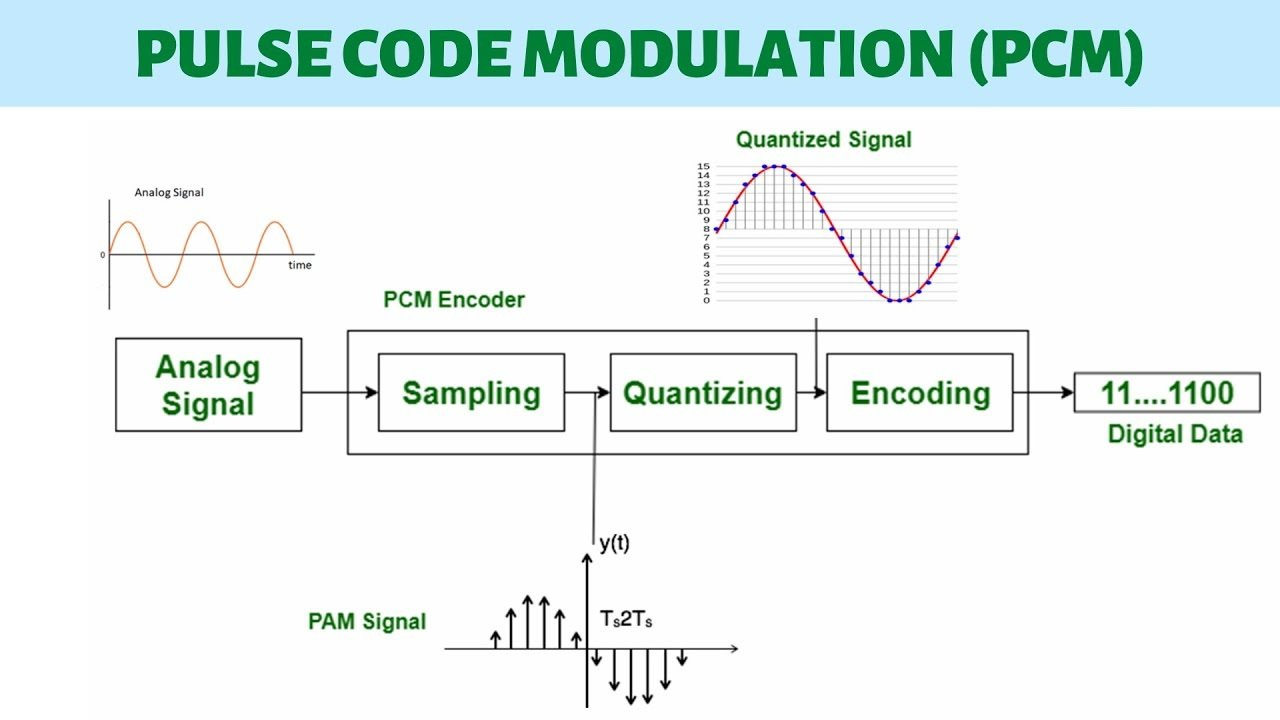
\includegraphics[width=\linewidth, keepaspectratio]{figures/pulse _code_modulation.jpg}
	\caption{Pulse Code Modulation (PCM) folyamat \cite{PULSECODEMODULATION}}
    \label{fig:pcm}
\end{figure}
%----------------------------------------------------------------------------
A digitális hangfeldolgozás területén fontos szerepet játszik az A/D átalakítók kialakítása, 
a kódolás folyamata, a D/A (digitális-analóg) átalakítás, valamint a hibafelismerés és hibajavítás.

A digitalizálási folyamat során az időbeli mintavételezés történik. 
Folyamatos mintavételezéskor a hang intenzitásával arányos diszkrét értékek, azaz feszültségimpulzusok jönnek létre. 
A mintavétel során az impulzusok a beérkező amplitúdó értékek alapján végtelen számú értéket vehetnek fel, 
ám a rendelkezésre álló bináris adatszók száma véges. Ezt a jelenséget kvantálásnak vagy tartományokba 
való felosztásnak nevezzük.

A kvantálás során a hangtartomány véges számú lépcsőre oszlik. 
A kvantálás finomsága, amely a mintavételi frekvenciával együtt a digitális jelfeldolgozás 
egyik legfontosabb paramétere, meghatározza a hang digitalizálásának részletességét. Gyakorlatilag a 
hangfrekvenciás jelek digitalizálásánál általában 14 vagy 16 bites kvantálást alkalmaznak. 
A kvantálásnál figyelembe kell venni a kvantálási zajt is, amely a tartományok növelésével csökkenthető.
A kvantálási zaj olyan zavaró tényező, amely a digitális hangrögzítés vagy -lejátszás során jelentkezik, 
és a kerekítési hibák következményeként alakul ki. Ez a zaj a különbség az eredeti analóg jel és a 
digitális formában ábrázolt jel értékei között, amit a digitális eszközök kvantálási folyamatában jelentkező pontatlanságok okoznak.
A kvantálási zaj keletkezése a digitális jel analóg formából történő diszkrét értékekre (kvantumokra) 
történő átalakítása során jelentkező kerekítési hibákra vezethető vissza. 
E hibák következtében a kvantálási zaj nemlineáris, hanem zavaró zajként észlelhető, 
amely nem harmonikus torzítás formájában jelenik meg, hanem inkább a hangminőség romlásához vezető zavaró tényezőként.

A kvantálási zaj csökkentésére több módszer létezik. Az egyik lehetséges megoldás a 
digitális jel dinamikatartományának növelése. Amennyiben a kvantálási pontosságot 
egy bittel növeljük, a jel-zaj viszony javulhat, és ezzel együtt a dinamika is +6 dB-el növekedhet. 
Továbbá, a zajcsökkentő algoritmusok alkalmazása és a magas felbontású digitális konverterek használata szintén hozzájárulhat a kvantálási zaj mérsékléséhez.
A kódolás során a hangszintek szerint kvantált pontok kódkombinációk sorozataként, digitális jelekként jelennek meg.
%----------------------------------------------------------------------------
\subsection{ADC és DAC konverterek - mintavételezés}
%----------------------------------------------------------------------------
A mintavételezés olyan folyamat, amely során egy analóg hangjelet digitális formába alakítanak át, azaz mintákat vesznek az időben folytonos hanghullámokból. 
Ez az alapja annak, hogy a hangot számítógépes rendszerekben kezelni lehessen. A hangminták gyakorisága meghatározza a mintavételi frekvenciát, 
ami meghatározza a digitális hangminőséget és a frekvencia tartományt. Általában minél magasabb a mintavételi frekvencia, annál jobb a hangminőség, 
de nagyobb sávszélességet is eredményez.

Az ADC (Analog-to-Digital Converter) konverter az analóg hangjelet digitális jelekké alakítja át, míg a DAC (Digital-to-Analog Converter) 
konverter a digitális jeleket visszaalakítja analóg hangjelekké. 
A professzionális ADC és DAC konverterek nagymértékben befolyásolják a hangminőséget.
%----------------------------------------------------------------------------
\section{Pontsugárzó hangforrás}
%----------------------------------------------------------------------------
A pontsugárzó hangforrások azok a hangfalak, amelyeket olyan módon modelleznek, mintha a hang egyetlen pontból származna, és a hangnyomás arányosan csökken a távolsággal. 
Ez a modell elsősorban olyan hangfalak esetében alkalmazható, amelyek önállóan működnek, például hangfalak dobozokban vagy mennyezetbe szerelve. 
Ezt a modellt főként olyan helyeken használják, ahol könnyen kell elérni a hangerősítést, például előadótermekben vagy kis koncerttermekben. 
Amikor több hangforrás kombinálódik, például kétutas hangfalrendszerekben, a transzducerek közötti kombináció bonyolultabb irányítottságot eredményez
a fizikai távolság és a szűrők kölcsönhatása miatt. 
Ennek eredményeként az irányítottság frekvenciától függően változik, ami kihívást jelent a hangrendszer tervezése során.
%----------------------------------------------------------------------------
\section{LineArray hangforrás}
%----------------------------------------------------------------------------
A LineArray hangforrások olyan hangfalrendszerek, amelyekben több hangdoboz egymás fölött van elrendezve, 
hogy egy közös lineáris hangforrást alkossanak. Ezt a technikát használják nagyobb hangosítási telepítéseknél, 
mivel egyetlen hangfal nem elegendő a szükséges hangteljesítmény eléréséhez és a közönségterület lefedéséhez. 
%----------------------------------------------------------------------------
\subsection{DSP-vezérelt irányítás}
%----------------------------------------------------------------------------
Az új generációs LineArray rendszereket DSP-kkel finomhangolják az egyes hangdobozok válaszának beállításához, lehetővé téve például
a függőleges irányítottság változtatását. Ez segít a hangot pontosan irányítani a közönség felé. 
A DSP-vezérelt hangszórórendszerek tervezése számítógépes eszközöket igényel, 
amelyek lehetővé teszik a hangszórók viselkedésének részletes szimulációját a teremmel összefüggésben, 
és optimalizálják a hangeloszlást a kívánt irányban.